\documentclass[article,aoas,preprint]{imsart}

\usepackage[nofiglist, nomarkers]{endfloat}
\usepackage{algorithm}
\usepackage{graphicx}
\usepackage{amsmath}
\usepackage{amssymb}
\usepackage{amsfonts}
\usepackage{amsthm}
\usepackage{xfrac}
\usepackage{float}
\usepackage{fullpage}
\RequirePackage[colorlinks,citecolor=blue,urlcolor=blue]{hyperref}

% override imsart settings for final project
\startlocaldefs
\setattribute{title}{size} {\fontseries{bx}\fontsize{14}{16}\selectfont\mathversion{bold}\spaceskip.5em}
\setattribute{journal}{name}{PH240F: Statistical Genomics II}
\setattribute{author}{prefix}{}
\setattribute{volume}{title}{Spring 2014---Final Project}

\makeatletter
\let\@fnsymbol\@arabic
\makeatother
\numberwithin{equation}{section}
\theoremstyle{plain}
\newtheorem{thm}{Theorem}[section]
\newtheorem{lemma}{Lemma}[section]
\newtheorem{definition}{Definition}
\newtheorem{Rule}{Rule}
\newtheorem*{notation}{Notation}
\endlocaldefs

% my standard setup 
\newcommand{\der}[2]{\frac{d #1}{d #2}} % for derivatives
\newcommand{\V}[1]{\ensuremath{\mathbf{#1}}} % for vectors
\newcommand{\gv}[1]{\ensuremath{\mbox{\boldmath$ #1 $}}} % for vectors of Greek letters
\newcommand{\pd}[2]{\frac{\partial #1}{\partial #2}}  % for partial derivatives
\newcommand{\grad}[1]{\gv{\nabla} #1} % for gradient
\newcommand{\reals}{\mathbb{R}}
\newcommand{\ints}{\mathbb{Z}}
\newcommand{\blank}{\underline{\hspace*{1in}}}
\newcommand{\PMF}{\mathrm{PMF}}
\newcommand{\PDF}{\mathrm{PDF}}
\newcommand{\CDF}{\mathrm{CDF}}
\newcommand{\N}[2]{\mathcal{N}\left(#1,#2\right)}
\newcommand{\empavg}[2]{\frac{1}{#1}\sum_{i=1}^{#1}\left[#2\right]}
\newcommand{\E}[1]{{\rm I\kern-.3em E}\left[#1\right]}
\newcommand{\Var}[1]{\mathrm{Var}\left[#1\right]}
\newcommand{\Cov}[1]{\mathrm{Cov}\left[#1\right]}
\def\ci{\perp\!\!\!\perp}
\newcommand{\argmax}[1]{\underset{#1}{\operatorname{argmax}}}
\newcommand{\argmin}[1]{\underset{#1}{\operatorname{argmin}}}
\newcommand{\iid}{\stackrel{\mathrm{iid}}{\sim}}
\newcommand{\logit}[1]{\operatorname{logit}({#1})}
\providecommand{\e}[1]{\ensuremath{\times 10^{#1}}}
\newcommand{\Tr}[1]{\mathrm{Tr}\left(#1\right)}
\newcommand{\adim}[2]{\underset{\scriptscriptstyle #1}{#2\strut}}

\newcommand{\fix}[1] { \textcolor{red} {
{\fbox{ {\bf Fix:} \ensuremath{\blacktriangleright }} {\bf #1}
\fbox{\ensuremath{\blacktriangleleft} } } } }



\begin{document}

\begin{frontmatter}

\title{Classification for Renal Cell Carcinomas}
\runtitle{Renal cell carcinomas classification}

\begin{aug}
\author{\fnms{Alex} \snm{Anderson},\thanksref{t1}\ead[label=e1]{aga@berkeley.edu}}
\author{\fnms{K. Jarrod} \snm{Millman},\thanksref{t2}\ead[label=e2]{millman@berkeley.edu}}
\and
\author{\fnms{Lara} \snm{Troszak}\thanksref{t2}\ead[label=e3]{troszak1@berkeley.edu}}
\thankstext{t1}{Department of Physics, UC Berkeley}
\thankstext{t2}{Division of Biostatistics, School of Public Health, UC Berkeley}
\runauthor{Anderson, Millman, and Troszak}
\end{aug}


\begin{abstract}

In this project, we compare classification methods for discriminating between
two different cancer cells. Specifically, we look at Kidney renal
papillary cell carcinoma (KIRP) and Kidney renal clear cell carcinoma (KIRC)
from the Cancer Genome Atlas.\footnote{\url{https://tcga-data.nci.nih.gov/tcga/}}

Using the unnormalized RNA-Seq expected count data from this website, we will
perform exploratory data analysis, looking at the need for normalization, low
count filtering, batch effects, and outlier removal.

Moving forward, we will utilize cross validation to assess our
classification methods. Using the training sets we rank the genes in terms
of differential expression between cell types based on their p-values.  These p-values 
are only utilized to rank the genes; we do not claim that they have any further meaning.
These ranks will be used for feature selection, comparing classification performance
based on different numbers of features (selection of the top 10, 20, 30, and 40
genes as features).

Finally, we perform several classification methods per feature set
(training our methods on the training data sets and testing our methods on the
validation data sets): Linear Discriminant Analysis, and
Support Vector Machines.  Additionally, we compare these methods to the
Random Forest classifier.

 
\end{abstract}

\begin{keyword}
\kwd{Renal Cell Carcinomas}
\kwd{Classification}
\kwd{Prediction}
\end{keyword}

\end{frontmatter}



\section{Introduction}

High throughput sequencing technology has revolutionized our ability to
understand how cells function, or in the case of cancer, malfunction. In this
study, we analyze RNA-Seq data from two types of renal cell carcinomas, clear and papillary. 
In this context, identifying a patient's cancer cell type informs the prognosis for the patient
and on how aggressively to treat the patient; clear cell carcinoma is considered the least likely to spread
and more likely to respond favorably to treatment. Therefore, our aim is to classify a patient's cancer type 
given their RNA-Seq expression data. To achieve this goal, we compare the accuracy of 
several classification methods.


\section{Methods}
\subsection{Classification Pipeline}

Starting from gene expression levels using the RSEM algorithm, we carried out
the following steps to analyze our data:

\begin{enumerate}
\item Split the data into training and validation sets. Two-thirds of our 72 subjects are allocated into the training set,
the rest are in the validation set.
\item Filter out genes with low average read counts for both cancer types in the training set. Specifically, if the 
mean expression count for a gene is less than 10 for both the KIRC and KIRP subjects, then the gene is filtered out of the training
set. After filtering, the number of genes we consider drops from $18,205$ to $17,136$.
\item Perform upper quantile normalization on the expression counts in the training set. The upper quantile of the normalized counts is stored and used to apply the training set's normalization to the test set counts.
\item Select features (i.e. genes) with which to train the classifiers in two ways:
\begin{itemize}
\item[-] Ranking the p-values from unequal sample size, unequal variance two-sided t-tests in the training set and selecting the genes with p-values below some threshold (i.e. picking the top 500 genes with the smallest p-values)
\item[-] Ranking the genes based on the variance of their expression counts across KIRC and KIRP subjects and selecting the
top genes with the largest variance.
\end{itemize}
\item Train several classifiers on the training data, with the selected features. Classifiers include Linear Discriminant Analysis, Support Machine Vectors, and Random Forest. Note that when training Random Forest, we include all of the genes instead of the just the selected features and allow it to make the decision on which genes best classify the two cancer cell types.
\item Filter and normalize the test data using the values from the second and third steps. 
\item Use the classifiers to predict cancer cell type for the subjects in the validation set.
\item Compare the accuracies of the predictions made by the classifiers by examining the proportion of correctly classified
subjects in the test set.
\end{enumerate}

\begin{figure}[H]
  \centering
    \includegraphics[width=.8\textwidth]{../../fig/rsem.png}
\caption{RSEM }
   \label{fig:rsem}
\end{figure}

\begin{figure}[H]
  \centering
    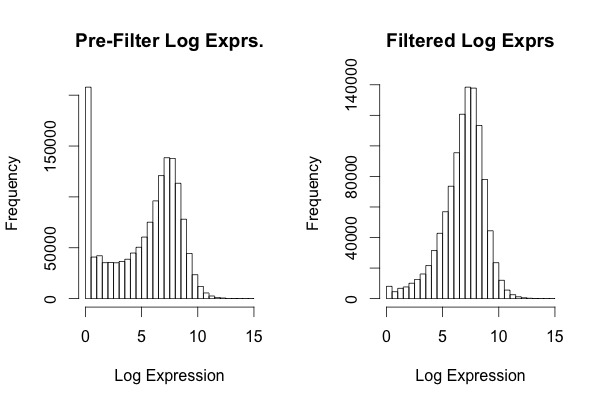
\includegraphics[width=\textwidth]{../../fig/filter_histograms.png}
\caption{Histogram }
   \label{fig:histogram}
\end{figure}

\begin{figure}[H]
  \centering
    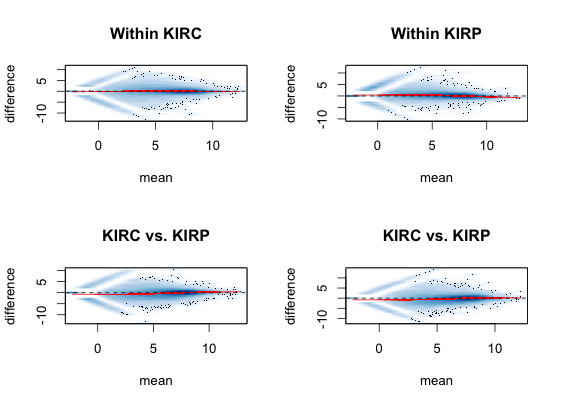
\includegraphics[width=\textwidth]{../../fig/mdplots_postnorm.png}
\caption{MD plots }
   \label{fig:mdplot}
\end{figure}

\begin{figure}[H]
  \centering
    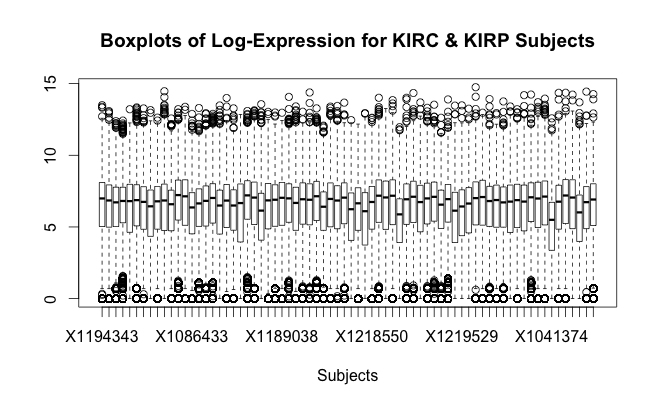
\includegraphics[width=\textwidth]{../../fig/postfilter_boxplot.png}
\caption{Boxplot }
   \label{fig:boxplot}
\end{figure}

\begin{figure}[H]
  \centering
    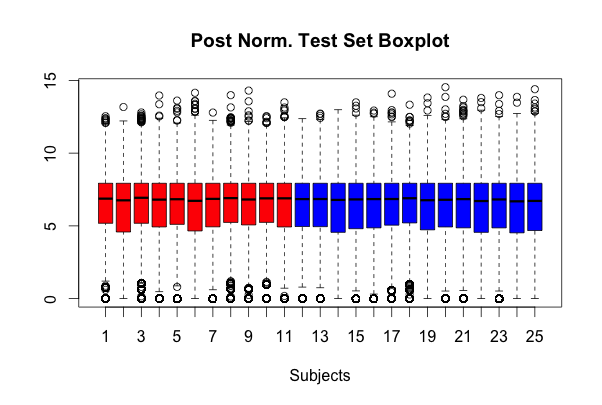
\includegraphics[width=.8\textwidth]{../../fig/postnorm_test_boxplot.png}
\caption{Boxplots after normalization }
   \label{fig:boxplotpost}
\end{figure}

\begin{figure}[H]
  \centering
    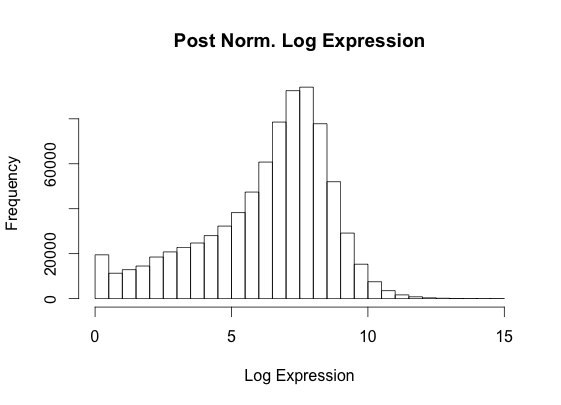
\includegraphics[width=.8\textwidth]{../../fig/postnorm_histogram.png}
\caption{Histogram after normalization  }
   \label{fig:histogram}
\end{figure}

\begin{figure}[H]
  \centering
    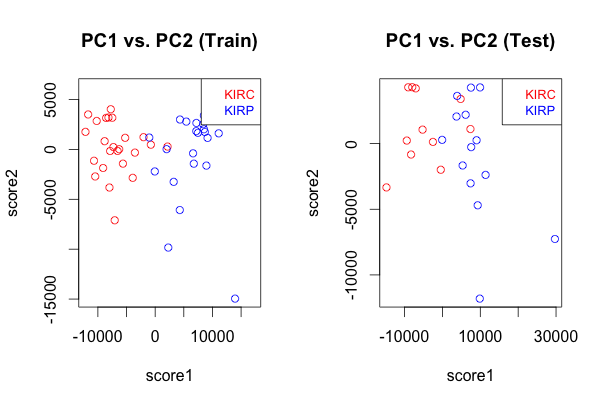
\includegraphics[width=.8\textwidth]{../../fig/pcplot.png}
\caption{PCA }
   \label{fig:pca}
\end{figure}


% Figure: histogram of gene expression after filtering. Looks reasonably normal. 
% Figure: box-plots of the normalized data
% Figure: mean difference plots after normalization
% Figure: mean difference plots after feature selection

Comments:

The t-test that we employed to do feature selection, also known as Welch's
t-test, used the following formula:

\begin{gather}
t = \frac{\overline{X}_1-\overline{X}_2}{s_{\overline{X}_1-\overline{X}_2}} \\
s_{\overline{X}_1-\overline{X}_2} = \sqrt{\frac{s_1^2}{n_1}+\frac{s_2^2}{n_2}} \\
\text{d.f.} = \frac{\left(\frac{s_1^2}{n_1}+\frac{s_2^2}{n_2} \right)}{\frac{s_1^4}{n_1^2(n_1-1)} + \frac{s_2^4}{n_2^2(n_2-1)}}
\end{gather}

\subsection{Classification Methods}

We investigated applied a number of methods in order to classify our data:

\begin{enumerate}
\item Principal Components Analysis - Choose the genes with the top X p-values. 
\item Support Vector Machines
\begin{itemize}
\item[-] SVM represents the training data as points in a space and maps them in a way
that the space between KIRC subjects and KIRP subjects is as wide as possible
\item[-] The validation data is then mapped into the same space. Predictions of cancer
cell type for these points are made based on which side of the dividing space that they fall. 
\end{itemize}
\item Linear Discriminant Analysis (with two clusters)
\begin{itemize}
\item[-] LDA finds the linear combination of genes, in our situation, which best separates our
training data into its two classes (KIRP and KIRC)
\item[-] This method is related to Principal Component Analysis; but differs in that LDA tries to
actually model the differences between categorical responses.
\end{itemize}
\item Random Forests
\begin{itemize}
\item[-] Random Forest builds numerous classification trees, each one constructed on a random subset of
features (genes), and predicts class based on the majority vote from all of the trees.
\end{itemize}
\end{enumerate}

\subsection{Performance Metrics}

Give our classification methods, we will consider a number of performance
metrics. We will look at accuracy (total correct over all predictions). Next,
for classifiers that give probabilities, we will plot the number of correct
predictions as a function of the number of false predictions for various
thresholds. Eg. if $p>t=0.1$, we say that we cannot decide which cancer type
that patient is. 

\section{Data}

The Cancer Genome Atlas (TCGA) collects and analyzes high-quality tumor samples
and makes a variety of data available online. We have downloaded RNA-Seq data
for two types of kidney cancer, KIRC and KIRP. The data was collected by the David
Neil Hayes group at UNC Chapel Hill. The data was produced using Illumina HiSeq
2000 sequencers. 

Counts per genes (GAF TCGA hg19 June 2011 build) calculated using the SeqWare
framework via the RSEM algorithm \cite{li2011rsem}.

While more data has been collected, we downloaded gene expression data from
$N_C =35$ patients with KIRC and $N_P = 37$ patients with KIRP.  For each
patient, we have gene expression data for $18,205$ genes. 

The data portal on TCGA website shows that subjects are organized into batches. A batch consists of
a group of subjects whose samples were processed together. Unfortunately,
we were unable to collect this information with the expression counts. Therefore, we are 
unable to examine possible batch effects that might obscure our feature selection. 

\section{Results}

After normalization and low read-count gene filtering, we attempt to select the best
genes to feed into the Support Vector Machines and Linear Discriminant Analysis classifiers.
We first produced a list of the genes with the largest variances across KIRC and KIRP subjects.
The top $N_best$ genes are presented in Table Y. Additionally, we produced a list of p-values
 for differential expression of genes in the two cancer types. Table X summarizes the genes with 
 the smallest p-values. Fig. Y shows a histogram of the p-values with lines showing typical 
 significance levels. 
 
As in Fig. X, we plotted the scores corresponding to the first two principal
components and colored the points according the cancer cell type. 
Evidently, the two cancer types separate nicely along the first
principal component. (Not too surprisingly since we ran this analysis using
only genes that were highly differentially expressed).  

%\begin{minipage}[c]{0.3\linewidth}
%\begin{quote}{\tiny  \ttfamily \raggedright \noindent
%~~~Variance~~~~~~~~~~~~~~~~~Tscore\\
%~\\
%~~~~~~true~~~~~~~~~~~~~~~~~~~~true\\
%pred~~~KIRC~KIRP~~~~~~~~pred~~~KIRC~KIRP\\
%~~KIRC~~~~7~~~~4~~~~~~~~~~KIRC~~~~8~~~~3\\
%~~KIRP~~~~4~~~10~~~~~~~~~~KIRP~~~~3~~~11
%}
%\end{quote}
%\end{minipage}
%\begin{minipage}[c]{0.3\linewidth}
%\begin{quote}{\tiny \ttfamily \raggedright \noindent
%~~~Variance~~~~~~~~~~~~~~~~~Tscore\\
%~\\
%~~~~~~true~~~~~~~~~~~~~~~~~~~~true\\
%pred~~~KIRC~KIRP~~~~~~~~pred~~~KIRC~KIRP\\
%~~KIRC~~~~7~~~~0~~~~~~~~~~KIRC~~~10~~~~0\\
%~~KIRP~~~~4~~~14~~~~~~~~~~KIRP~~~~1~~~14
%}
%\end{quote}
%\end{minipage}
%\begin{minipage}[c]{0.3\linewidth}
%\begin{quote}{\tiny \ttfamily \raggedright \noindent
%~\\
%~\\
%~~~~~~true\\
%pred~~~KIRC~KIRP\\
%~~KIRC~~~~8~~~~0\\
%~~KIRP~~~~3~~~14
%}
%\end{quote}
%\end{minipage}






\section{Discussion}

Our results are fundamentally limited due to the data. As this data was not
designed for this type of experiment, necessary controls are not in place. For
instance, the differences between gene expression may be due to technical
effects. We do not have batch information for the subjects, so we cannot try 
to correct for possible batch effect. Fig. Z shows Mean-Difference Plots of
subjects within the same cancer cell type and of subjects with differing cell types.
This is problematic because differences in expression between groups may be 
due to technical effects as opposed to biological effects of interest. In our feature 
selection, we might be unknowingly, choosing genes on which to build the classifiers
that reflect the technical effects, and not those that reflect biological differences between
subjects with KIRC and KIRP.
From these plots, we see that the magnitude of technical effects within a cell type
is similar to the magnitude of the biological effects between cell types which interest
us. Also, the RNA-Seq experiments were 
carried out a few months apart. It is not clear what efforts were made to 
standardize the procedure of processing the cancer samples. In the future, 
it would be important to have a negative control where two samples that are 
supposed to be the same are processed at during the two times that the cancer 
cells were processed. 

Nonetheless, all of our classification methods appear to satisfactorily predict 
cancer cell type in new patients, given their expression in some selected genes. The classifiers
using the subset of genes determined by ranked p-values performed slightly better than the classifiers
built with the subset of genes with the largest variances.

The proportion of correctly classified subjects for each of the methods using the smallest p-value subset of
genes is as follows:
\begin{enumerate}
\item Support Vector Machine - $Accuracy = 96\%$
\item Linear Discriminant Analysis - $Accuracy = 76\%$
\end{enumerate}

The proportion of correctly classified subjects for each of the methods using the largest variance subset of
genes is as follows:
\begin{enumerate}
\item Support Vector Machine - $Accuracy = 84\% $
\item Linear Discriminant Analysis - $Accuracy =68\% $
\end{enumerate}

Random Forest is not built on a subset of the genes in our dataset, but rather all of the genes. It is allowed
to determine the best subset of genes for classification of cell type. The proportion of correctly 
classified validation subjects using Random Forest is $88\%$.

The classifier that best predicts cancer cell types in the validation set is Support Vector Machine, 
correctly predicting for $24$ out of $25$ subjects.

In the future,  it may be interesting to compare different ways of normalizing the data. For instance,
we chose upper quantile normalization for our analysis due to its frequent use and because it alter 
count distributions as radically as full quantile normalization.


\section*{Acknowledgments}

We would like to thank Davide Risso for pointing us to the Cancer Genome Atlas
as well as providing feedback on our proposal. Sandrine Dudoit and Haiyan Huang
offered us important feedback on our initial proposals as well as on our
intermediate results. 

\bibliographystyle{imsart-number} %bibliographystyle{imsart-nameyear}
\bibliography{kidney}

\end{document}
